\section{Design}
In questa fase si descrive la fase di progettazione del sistema dal punto di vista del design, costruendo il database, elencando le tecnologie utilizzate e presentando un architettura del completa del sistema.
\subsection{Architettura del Sistema}
PocketDev presenta un'architettura client server in 3 tier. Il primo è rappresentato dal database TDB adatto a memorizzare triplette in formato RDF in maniera efficiente e compatta. Nel secondo abbiamo la logica di business suddivisa in 2 componenti principali: il componente \textbf{Fuseki} che interroga il Database tramite Query SPARQL restituendo dei JSON e il \textbf{Server} che prende questi risultati, li formatta e li spedisce al terzo tier. Quest'ultimo comunica con il secondo con un interfaccia REST sempre tramite JSON e il componente \textbf{Browser} li renderizza a schermo. 
\begin{figure}[H]
 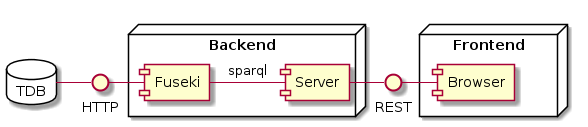
\includegraphics[scale=.6]{architecture.png}
\end{figure}
\subsection{Definizione del Database}
Il database non è il solito database relazionale, ma un database di tipo semantico dove le informazioni vengono memorizzate attraverso triplette di concetti. Queste triplette sono composte da 3 componenti: soggetto, predicato ed oggetto. Alla base dell'ontologia di PocketDev ci sono i seguenti concetti:
\begin{enumerate}
 \item IT\_Career: è il concetto che esprime la carriera universitaria;
 \item Educational\_Path: è il percorso formativo che un utente segue per prepararsi alla carriera desiderata;
 \item TheoryEducationalPath: insieme di elementi di Educational\_Path riguardanti aspetti teorici del percorso formativo. Essi si dividono a sua volta in Base, Intermediate ed Advanced.
 \item PraticalEducationalPath: insieme di elementi di Educational\_Path rigurdanti aspetti pratici del percorso formativo. Si divide a sua volta in:
 \begin{enumerate}
  \item Language: insieme di linguaggi di programmazione;
  \item Editor: strumenti di editing che supportano vari tipi di linguaggi;
  \item Coding: strumenti di support alla fase di coding;
  \item Design: strumenti di supporto al design;
  \item Versioning: strumnti di supporto al versioning;
  \item Library: insieme di librerie famose;
 \end{enumerate}
 \item support: funzione che associa un editor ad uno o più linguaggi di programmazione.
 \item dependsOn: funzione che associa un concetto teorico ad un altro;
 \item generated: funzione che associa una linguaggio ad una libreria.
 \item follow: funzione che associa una carriera ad un centto teorico avanzato.
\end{enumerate}
L'idea delle associazioni è la seguente: per raggiungere una carriera bisogna conoscere dei concetti pratici ma soprattutto dei concetti teorici avanzati. Questi ultimi a loro volta necessitano di concetti teorici intermedi per essere appresi e infine a loro volta di concetti di base.
\subsection{Popolazione}
La popolazione dell'ontologia è stata effettuata in modo semiautomatico. Tutti gli individui di ogni concetto sono stati prelevati da DBPedia e quindi è stato usato il loro IRI per poter ricavare le informazioni di base. Ogni individuo a sua volta è stato decorato con l'aggiunta di nuove informazione per rendere il dato più ricco e uniforme agli obiettivi del progetto. 
\begin{enumerate}
 \item hasName: un nome univoco per poter visualizzare in maniera umanamente comprensibile, il concetto su schermo;
 \item hasGuide: un URI che punta alla pagina di una guida di \textit{tutorialspoint} di un concetto teorico o pratico che viene  parsata dal nostro client e renderizzata sulla pagina di PocketDev;
 \item hasBooks: un URI che punta ad una pagina che contiene un insieme di libri consigliati per approfondire il concetto teorico/pratico anch'esso parsato e renderizzato sulla pagina di PocketDev.
\end{enumerate}
